%% LyX 2.1.4 created this file.  For more info, see http://www.lyx.org/.
%% Do not edit unless you really know what you are doing.
\documentclass[english,nohyper]{tufte-handout}
\usepackage[T1]{fontenc}
\usepackage[latin9]{inputenc}
\usepackage{amsmath}
\usepackage{amssymb}
\usepackage{graphicx}

\makeatletter

%%%%%%%%%%%%%%%%%%%%%%%%%%%%%% LyX specific LaTeX commands.

\title{Visual-Inertial Extended Kalman Filter\\
Using Manifold Representations}
\author{James Jackson and Robert Pottorff}

\makeatother

\usepackage{babel}
\begin{document}
\maketitle
\global\long\def\q{\boldsymbol{q}}


\global\long\def\xhat{\mathbf{\hat{\mathbf{x}}}}


\global\long\def\dxhat{\hat{\dot{\mathbf{x}}}}


\global\long\def\x{\mathbf{x}}


\global\long\def\u{\mathbf{u}}



\section{Introduction}

Monocular Visual-Inertial Navigation is an important topic for autonomous
robots. Miniature Aerial Vehicles (MAVs) in particular often benefit
from vision-aided navigation but are limited in size, weight and power.
Kalman Filter approaches are often utilized to provide state and velocity
estimates given sensor measurements from an IMU and camera pair. These
sensors are often augmented with laser range finders, sonars, and
image depth measurements, such as from an RGB-D camera to provide
additional information to improve state estimates.

In many real-life robotics problems, the attitude of the robot cannot
be represented simply. Many modern approaches use a quaternion to
represent the attitude of the robot. Quaternions provide computational
efficiency and do not suffer from singularities, but they are over-parameterized
and do not form a vector space. Many approaches, such as the Multiplicative
Extended Kalman Fiter (MEKF) utilize an ``error state'' parameterization,
and some manipulation is performed to guarantee that covariance estimates
and measurement updates are applied to an error state, which can be
considered as a true vector, about some reference trajectory, which
is represented with a full quaternion.

\citet{Hertzberg2013} illustrates a new method to deal with the non-vector
elements of a estimator state by introducing the $\boxplus$ and $\boxminus$
operators, which abstract the mathematics of operating on group elements
to make it possible to homongenize the use of vector and non-vector
elements in an estimator state. We will use this method to simplify
the derivation and implementation of our filter. We also will use
quaternions to represent estimated bearings to observed features in
the camera frame as shown by \citet{Bloesch2015a}, accompanied by
our own explanation for how this parameterization works. We have also
included the relevant jacobian definitions and measurement models
for feature measurements, depth measurements to features (i.e. from
an RGBD camera), altimeter, accelerometer, position, velocity, attitude,
and pixel velocity (as calculated by optical flow) required for a
complete implementation of this filter.

The objective of this report is to simply and accurately describe
everything required for an extended Kalman Filter operating directly
on the manifold using the $\boxplus$ and $\boxminus$ operators,
applied to multirotor dynamics as described by \citet{Leishman2014b}.
In addition, we will describe the results of experiments of this filter
on a multirotor robot using operating in a GPS-denied environment.


\section{Notation}

For this report, we will use the following notation for describing
coordinate frames

\[
\begin{aligned}q_{i}^{b} & \quad\textrm{Quaternion describing rotation from the inertial frame to the body frame}\\
v_{b/i}^{b} & \quad\textrm{velocity of the body frame, with respect to the inertial frame, expressed in the body frame}\\
p_{bi}^{i} & \quad\textrm{position of the body, with respect to the inertial frame, expressed in the inertial frame}
\end{aligned}
\]
.

We will also make extensive use of the skew-symmetric matrix, defined
as

\[
\left\lfloor v\right\rfloor =\left[\begin{array}{ccc}
0 & -v_{3} & v_{2}\\
v_{3} & 0 & -v_{1}\\
-v_{2} & v_{1} & 0
\end{array}\right]
\]


which is related to taking cross-product between two vectors, that
is
\[
v\times w=\left\lfloor v\right\rfloor w
\]
.

All quaternions used in this report use a Hamiltonian (right-handed)
convention are assumed to be unit norm, and will be expressed as column
vectors as shown below. 
\[
q=q_{w}+q_{x}i+q_{y}j+q_{z}k=\begin{bmatrix}q_{w}\\
\bar{q}
\end{bmatrix}
\]
The use of Hamiltonian quaternions result in multiplication being
defined as

\[
p\otimes q=\begin{bmatrix}p_{w} & -\bar{p}^{\top}\\
\bar{p} & p_{w}I_{3\times3}+\left\lfloor \bar{p}\right\rfloor 
\end{bmatrix}\begin{bmatrix}q_{w}\\
\bar{q}
\end{bmatrix}
\]
.

The $3\times3$ Rotation matrix $R\left(q\right)$ based on this quaternion
is defined as follows

\[
R\left(q\right)=\left(2q_{w}^{2}-1\right){\bf I}-2q_{w}\left\lfloor \bar{q}\right\rfloor +2\bar{q}\bar{q}^{\top}\in\mathbb{R}^{3\times3}
\]


and describes a passive rotation. That is $R\left(q\right)v$ will
result in the original vector $v$, represented in a new coordinate
frame described by $R\left(q\right)$. The active rotation $R^{\top}\left(q\right)v$
results in a new rotated object expressed in the original frame.

The exponential mapping of the quaternion is shown in Equations \ref{eq:quaternion_exp}
and \ref{eq:quaternion_log}. For numerical stability, we will also
utilize the associated linearization for very small rotations, (with
magnitude less than 1e-4). These mappings are used to convert to and
from the Lie algebra associated with the quaternion group. In Lie
tangent space, quaternion multiplication can be performed as vector
addition, which ultimately allows us to define a covariance matrix
about a non-vector quaternion object.

\begin{equation}
\begin{aligned}\exp\left(\boldsymbol{\delta}\right) & =\begin{bmatrix}\cos\left(\frac{\lVert\delta\rVert}{2}\right)\\
\sin\left(\frac{\lVert\delta\rVert}{2}\right)\frac{\delta}{\lVert\delta\rVert}
\end{bmatrix}\\
 & \approx\left[\begin{array}{c}
1\\
\frac{\delta}{2}
\end{array}\right]
\end{aligned}
\label{eq:quaternion_exp}
\end{equation}


\begin{equation}
\begin{aligned}\log\left(q\right) & =2\mathrm{atan2}\left(\left\Vert \bar{q}\right\Vert ,q_{w}\right)\frac{\bar{q}}{\left\Vert \bar{q}\right\Vert }\\
 & \approx2\textrm{sign}\left(q_{w}\right)\bar{q}
\end{aligned}
\label{eq:quaternion_log}
\end{equation}


The will use the following $\boxplus$ and $\boxminus$ operators
for operating on the rotation manifold within our kalman filtering
framework. 

\begin{align}
\boxplus & :SO\left(3\right)\times\mathbb{R}^{3}\rightarrow SO\left(3\right)\nonumber \\
 & q,\theta\mapsto q\otimes\exp\left(\theta\right)\\
\boxminus & :SO\left(3\right)\times SO\left(3\right)\rightarrow\mathbb{R}^{3}\nonumber \\
 & q,p\mapsto\log\left(p^{-1}\otimes q\right)
\end{align}
These operators, as described in \citet{Hertzberg2013}, abstracts
the Lie algebra manipulation and allows us to consider Quaternions
and vectors homogenously. As a specific example, they can be used
to add rotation pertubations to quaternions and to difference quaternions
as shown below

\begin{eqnarray*}
q_{t+1} & = & q_{t}\boxplus\theta\\
\theta & = & q_{1}\boxminus q_{2}
\end{eqnarray*}



\section{Bearing Vectors}

We have to find some way to parameterize the bearing vectors to features
using the $\boxplus$ and $\boxminus$ operators. While the most obvious
parameterization would seem to be unit vectors on $S^{2}$, there
is no way to define a set of orthonormal vectors which span the space
such that a suitable difference operator can be defined.

Instead, we will use rotations in $SE(3)$ to define the representation.
Let $\zeta_{i}$ be the 3D unit vector directed at feature $i$, with
respect to the camera frame $\mathcal{C}$. We then define $q_{C}^{\zeta_{i}}$as
the quaternion rotation between $e_{z}$, the z-axis of the camera
frame and the 3D unit bearing vector$\zeta_{i}$. The change between
two 3D unit vectors $\zeta_{i}$ and $\zeta_{j}$ can be described
using an axis-angle representation, where the direction of the axis
of rotation is perpendicular to the 3D unit vectors, and is scaled
by the angle. This is illustrated in Figure \ref{fig:bearing_vector_geometry}.

\begin{figure}
\begin{centering}
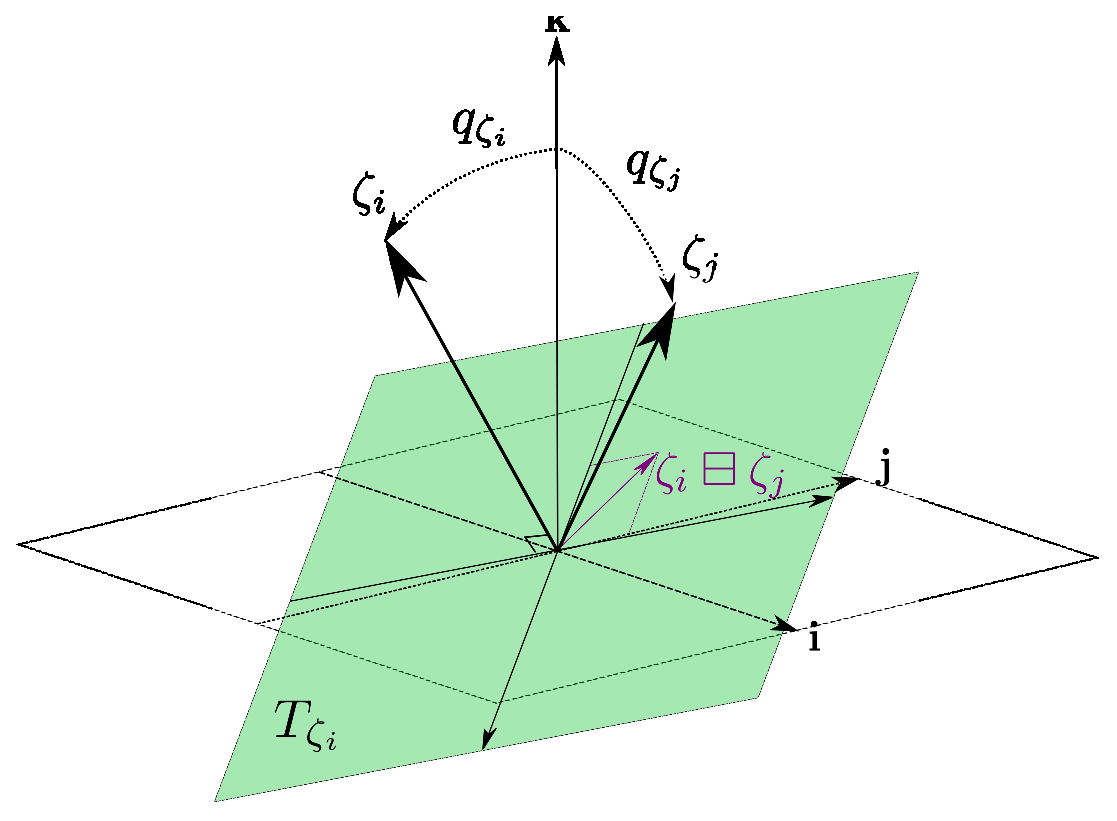
\includegraphics[width=0.8\columnwidth]{figures/feature_diagram}
\par\end{centering}

\label{fig:bearing_vector_geometry}

\caption{Illustration of Bearing Vector Geometry}
\end{figure}


As can be seen in the picture, there are only 2 degrees of freedom
in this parameterization because the axis of rotation is always in
the plane normal to $\zeta_{i}$. Therefore, we can define a projection
matrix $T_{\zeta}$, which reduces the dimensionality of the axis-angle
representation to this plane. 

\begin{equation}
\boldsymbol{\zeta}=R\left(q_{c}^{\zeta}\right)^{\top}\boldsymbol{e}_{z}\in\mathcal{S}^{2}\subset\mathbb{R}^{3}
\end{equation}


\begin{equation}
T_{\zeta}=R\left(q_{c}^{\zeta}\right)^{\top}\left[\begin{array}{cc}
\boldsymbol{e}_{x} & \boldsymbol{e}_{y}\end{array}\right]\in\mathbb{R}^{3\times2}
\end{equation}


Using this parameterization, we can now define the $\boxplus$ and
$\boxminus$ operators of this space.

\begin{align}
\boxplus & :SO\left(3\right)\times\mathbb{R}^{2}\rightarrow SO\left(3\right),\nonumber \\
 & \boldsymbol{q}_{\zeta},\boldsymbol{u}\mapsto\exp(T_{\zeta}\boldsymbol{u})\otimes\boldsymbol{q}_{\zeta},\label{eq:feat_boxplus}\\
\boxminus & :SO\left(3\right)\times SO\left(3\right)\rightarrow\mathbb{R}^{2},\nonumber \\
 & \boldsymbol{q}_{\zeta_{i}},\boldsymbol{q}_{\zeta_{j}}\mapsto T_{\zeta_{j}}^{\top}\theta s\left(q_{\zeta_{i}},q_{\zeta_{j}}\right),\label{eq:feat_boxminus}
\end{align}


where $\theta$ is the angle between the two unit bearing vectors
$\zeta_{i}$ and $\zeta_{j}$
\begin{equation}
\theta=\cos^{-1}\left(\zeta_{i}^{\top}\zeta_{j}\right)
\end{equation}


and 

\begin{equation}
s\left(q_{\zeta_{i}},q_{\zeta_{j}}\right)=\dfrac{\zeta_{j}\times\zeta_{i}}{\lVert\zeta_{j}\times\zeta_{i}\rVert}
\end{equation}


is the axis of rotation.

Unlike attitude quaternions, there are only two degrees of freedom
associated with feature bearings. This results in an infinite number
of quaternions which can describe the same $\zeta$ bearing vector.
This parameterization departs slightly from the requirements specified
by \citet{Hertzberg2013}, but still sufficiently represents feature
bearings on the smooth $SE\left(3\right)$ manifold. Intuitively speaking,
we do not care about any rotation about the feature bearing vector,
but the quaternion representaiton may accumulate it. Because the difference
operator operates primarily on the $\zeta$ vectors between two quaternions,
the freewheeling dimension in the quaternion representation is mapped
to the null space, and the difference is unambiguous, despite having
an extra degree of freedom.


\section*{Continuous-Discrete EKF Equations}

Using the parameterizations above, we can now define the continuous-discrete
EKF framework, using the manifold represenations and the $\boxplus$/$\boxminus$
abstraction.


\subsection{Prediction}

The state and covariance dynamics are shown in Equation \ref{eq:prediction_step}. 

\begin{equation}
\begin{aligned}\dxhat & =f\left(\xhat,\mathbf{\u}\right)\\
A & =\left.\frac{\partial f}{\partial\x}\right|_{\x=\xhat}\\
G & =\left.\frac{\partial f}{\partial\u}\right|_{\x=\xhat}\\
\dot{P} & =AP+PA^{\top}+GQ_{\u}G+Q_{\x}
\end{aligned}
\label{eq:prediction_step}
\end{equation}


These dynamics can be integrated using euler integration on the manifold
with 

\begin{equation}
\begin{aligned}\xhat\left(t\right) & =\xhat\left(t-dt\right)\boxplus\dot{\x}dt\\
P\left(t\right) & =P\left(t-dt\right)+\dot{P}dt
\end{aligned}
\end{equation}



\subsection{Update for Measurement $y$}

Equation \ref{eq:update_step} is a direct update on the manifold
for some measurement model $h_{y}\left(\x\right)$.

\begin{equation}
\begin{aligned}H_{y} & =\frac{\partial h_{y}}{\partial\x}\\
K & =PH_{y}^{\top}\left(R_{y}+HPH^{\top}\right)^{-1}\\
P^{+} & =(I-KH_{y})P^{-}\\
\hat{\x}^{+} & =\hat{\x}^{-}\boxplus K\left(\mathbf{z}_{y}\boxminus h_{y}\left(\hat{\x}\right)\right)
\end{aligned}
\label{eq:update_step}
\end{equation}



\section{State Definition}

For the multirotor agent, we define the estimator state as follows:

\[
\begin{aligned}p_{bI}^{I} & \quad\textrm{position of MAV body frame w.r.t. inertial frame, expressed in inertial frame}\\
v_{b/I}^{b} & \quad\textrm{velocity of MAV w.r.t. inertial frame, expressed in the body frame}\\
q_{I}^{b} & \quad\textrm{rotation from inertial to body frame, expressed in the inertial frame as a unit quaternion}\\
\beta_{a} & \quad\textrm{accelerometer constant bias}\\
\beta_{\omega} & \quad\textrm{rate gyroscope constant bias}\\
\mu & \quad\textrm{constant linear drag term}\\
q_{c}^{\zeta_{i}} & \quad\textrm{rotation from the camera z axis to the unit bearing vector directed at feature }i\textrm{ expressed in the camera frame as a unit quaternion}\\
\rho_{i} & \quad\textrm{inverse depth to feature }i
\end{aligned}
\]


\[
\boldsymbol{x}=\left[p_{bI}^{I},v_{b/I}^{b},q_{I}^{b},\beta_{a},\beta_{\omega},\mu,q_{c}^{\zeta_{0}}\cdots q_{c}^{\zeta_{n}},\rho_{0}\cdots\rho_{n}\right]^{\top}
\]
Where $x$ is a $17+5n$ vector.

The covariance matrix $P$, which is defined as 
\[
P=E\left[\hat{\boldsymbol{x}}\boxminus\boldsymbol{x}\right]E\left[\hat{\boldsymbol{x}}\boxminus\boldsymbol{x}\right]^{\top}
\]
is a $\left(16+3n\right)\times\left(16+3n\right)$ matrix, due to
the nature of the $\boxminus$ operator and the underlying parameterization
of $\boldsymbol{x}$

The system is mechanized using IMU sensor measurements $y_{a}$ and
$y_{\omega}$

\[
\begin{aligned}\boldsymbol{u} & =\left[\begin{array}{c}
y_{a}\\
y_{\omega}
\end{array}\right]\end{aligned}
\in\mathbb{R}^{6\times1}
\]



\section{Dynamics}

Now that we have defined all the relevant parameterizations, we can
define the dynamics for our system. We will use generic rigid-body
dynamics mechanized by acceleration and angular velocity inputs $\boldsymbol{y}_{a}$
and $\boldsymbol{y}_{\omega}$ respectively. A rigorous derivation
of feature bearing vector and depth dynamics are given in the appendix.

\begin{equation}
\begin{aligned}\dot{p}_{bI}^{I} & =R^{\top}\left(q_{I}^{b}\right)v_{bI}^{b}\\
v_{b/I}^{b} & =R\left(q_{I}^{b}\right)^{\top}g+\left[\begin{array}{ccc}
0 & 0 & 0\\
0 & 0 & 0\\
0 & 0 & 1
\end{array}\right]\left(y_{a}-\beta_{a}\right)-\mu_{t}\left[\begin{array}{ccc}
1 & 0 & 0\\
0 & 1 & 0\\
0 & 0 & 0
\end{array}\right]v_{b/I}^{b}+\eta_{v}\\
\dot{q}_{I}^{b} & =y_{\omega}-\beta_{\omega}\\
\dot{\beta}_{a} & =\eta_{\beta_{a}}\\
\dot{\beta}_{\omega} & =\eta_{\beta_{\boldsymbol{\omega}}}\\
\dot{\mu} & =\eta_{\mu}\\
\dot{q}_{c}^{\zeta_{i}} & =T_{\zeta}^{\top}\left(-\rho_{i}\left\lfloor \zeta_{i}^{c}\right\rfloor \left(v_{c/I}^{c}\right)+\omega_{c/I}^{I}\right)\\
\dot{\rho_{i}} & =\rho_{i}^{2}\left(\zeta_{i}^{c}\right)^{\top}v_{c/I}^{c}
\end{aligned}
\label{eq:full_dynamics}
\end{equation}



\section{State Jacobians	}

We now want the derivative of the state propagation function with
respect to the state $F=\frac{\partial\dot{\boldsymbol{x}}}{\partial\boldsymbol{x}}$. 

\[
F=\left[\begin{array}{ccccccccc}
0 & R\left(q_{I}^{b}\right)^{\top} & \left\lfloor v_{bI}^{b}\right\rfloor  & 0 & 0 & 0 & \cdots & 0 & 0\\
0 & -\mu\left[\begin{array}{ccc}
1 & 0 & 0\\
0 & 1 & 0\\
0 & 0 & 0
\end{array}\right] & -\left\lfloor R\left(q_{I}^{b}\right)g\right\rfloor  & -\hat{k}\hat{k}^{\top} & 0 & \left[\begin{array}{ccc}
1 & 0 & 0\\
0 & 1 & 0\\
0 & 0 & 0
\end{array}\right]v_{b/I}^{b} & \cdots & 0 & 0\\
0 & 0 & 0 & 0 & 0 & -I_{3\times3} & \cdots & 0 & 0\\
0 & 0 & 0 & 0 & 0 & 0 & \cdots & 0 & 0\\
0 & 0 & 0 & 0 & 0 & 0 & \cdots & 0 & 0\\
0 & 0 & 0 & 0 & 0 & 0 & \cdots & 0 & 0\\
\vdots & \vdots & \vdots & \vdots & \vdots & \vdots & \ddots & \vdots & \vdots\\
0 & 0 & 0 & 0 & \dfrac{\partial\dot{q}_{c}^{\zeta_{i}}}{\partial\beta_{\omega}} & 0 & \cdots & \dfrac{\partial\dot{q}_{c}^{\zeta_{i}}}{\partial q_{c}^{\zeta_{i}}} & \dfrac{\partial\dot{q}_{c}^{\zeta_{i}}}{\partial\rho_{i}}\\
0 & \dfrac{\partial\dot{\rho}_{i}}{\partial v_{b/i}^{i}} & 0 & 0 & \dfrac{\partial\dot{\rho}_{i}}{\partial\beta_{\omega}} & 0 & \cdots & \dfrac{\partial\dot{\rho}_{i}}{\partial q_{c}^{\zeta_{i}}} & \dfrac{\partial\dot{\rho}_{i}}{\partial\rho_{i}}
\end{array}\right]
\]


\[
\begin{aligned}\dfrac{\partial\dot{q}_{c}^{\zeta_{i}}}{\partial\beta_{\omega}} & =T_{\zeta}^{\top}\left(\rho_{i}\left\lfloor \zeta_{i}^{c}\right\rfloor R\left(q_{b}^{c}\right)\left\lfloor p_{cb}^{b}\right\rfloor -R\left(q_{b}^{c}\right)\right)\end{aligned}
\]


\[
\begin{aligned}\dfrac{\partial\dot{q}_{c}^{\zeta_{i}}}{\partial q_{c}^{\zeta_{i}}} & =-T_{\zeta}^{\top}\left(\left\lfloor \rho_{i}\left\lfloor v_{c/i}^{c}\right\rfloor \zeta_{i}^{c}+\omega_{c/i}^{c}\right\rfloor +\left(\rho_{i}\left\lfloor v_{c/i}^{c}\right\rfloor \left\lfloor \zeta_{i}^{c}\right\rfloor \right)\right)T_{\zeta}\end{aligned}
\]


\[
\begin{aligned}\dfrac{\partial\dot{q}_{c}^{\zeta_{i}}}{\partial\rho_{i}} & =T_{\zeta}^{\top}\left\lfloor \zeta_{i}^{c}\right\rfloor v_{c/i}^{c}\end{aligned}
\]


\[
\begin{aligned}\frac{\partial\dot{\rho_{i}}}{\partial v_{b/i}^{i}} & =\rho_{i}^{2}\left(\zeta_{i}^{c}\right)^{\top}R\left(q_{b}^{c}\right)\end{aligned}
\]


\[
\begin{aligned}\frac{\partial\dot{\rho_{i}}}{\partial\beta_{\omega}} & =\rho_{i}^{2}\left(\zeta_{i}^{c}\right)^{\top}R\left(q_{b}^{c}\right)\left\lfloor p_{cb}^{b}\right\rfloor \end{aligned}
\]


\[
\begin{aligned}\frac{\partial\dot{\rho_{i}}}{\partial q_{c}^{\zeta_{i}}} & =\rho_{i}^{2}\left(v_{c/i}^{c}\right)^{\top}\left\lfloor \zeta\right\rfloor T_{\zeta}\end{aligned}
\]


\[
\begin{aligned}\frac{\partial}{\partial\rho_{i}}\dot{\rho_{i}} & =2\rho_{i}\left(\zeta_{i}^{c}\right)^{\top}v_{c/i}^{c}\end{aligned}
\]



\section{Input Jacobians}

Now, we want the jacobian for mapping $G=\frac{\partial\dot{\boldsymbol{x}}}{\partial\boldsymbol{u}}$

\[
G=\left[\begin{array}{ccccccccc}
0 & \hat{k}\hat{k}^{\top} & 0 & 0 & 0 & 0 & \cdots & 0 & 0\\
0 & \left\lfloor v_{b/I}^{b}\right\rfloor  & -I_{3\times3} & 0 & 0 & 0 & \cdots & \dfrac{\partial\dot{q}_{c}^{\zeta_{i}}}{\partial y_{\omega}} & \dfrac{\partial\dot{\rho}_{i}}{\partial y_{\omega}}
\end{array}\right]
\]


\[
\begin{aligned}\dfrac{\partial\dot{q}_{c}^{\zeta_{i}}}{\partial y_{\omega}} & =T_{\zeta}^{\top}\left(R\left(q_{b}^{c}\right)-\rho_{i}\left\lfloor \zeta_{i}^{c}\right\rfloor R\left(q_{b}^{c}\right)\left\lfloor p_{cb}^{b}\right\rfloor \right)\end{aligned}
\]


\[
\begin{aligned}\frac{\partial\dot{\rho_{i}}}{\partial y_{\omega}} & =\rho_{i}^{2}\left(\zeta_{i}^{c}\right)^{\top}R\left(q_{b}^{c}\right)\left\lfloor p_{cb}^{b}\right\rfloor \end{aligned}
\]



\section{Measurement Models}


\subsection{Accelerometer}

\[
\begin{aligned}h_{acc}\left(x,u,\eta_{a}\right) & =I_{2\times3}\left(-\mu v_{b/i}^{b}+\beta_{a}+\eta_{a}\right)\end{aligned}
\]


\[
H_{acc}=\left[\begin{array}{ccccccccc}
0 & -\mu I_{2\times3} & 0 & I_{2\times3} & 0 & -I_{2\times3}v_{b/i}^{b} & \cdots & 0 & 0\end{array}\right]
\]



\subsection{Altimeter}

Assuming a flat earth, the altimeter directly measures altitude

\[
\begin{aligned}h_{alt}(x, & u,\eta_{alt})\end{aligned}
=-\hat{k}^{\top}p_{bI}^{I}+\eta_{alt}
\]


\[
\begin{aligned}\frac{\partial h_{alt}}{\partial x} & =\left[\begin{array}{cccccccc}
-\hat{k}^{\top} & 0 & 0 & 0 & 0 & 0 & 0\cdots0 & 0\cdots0\end{array}\right]\end{aligned}
\]



\subsection{Feature Point}

We assume that we have a known camera calibration matrix of the following
form

\[
\begin{aligned}K & =\left[\begin{array}{ccc}
f_{x} & s & x_{0}\\
0 & f_{y} & y_{0}\\
0 & 0 & 1
\end{array}\right]\end{aligned}
\]


Which maps world $\left[\begin{array}{ccc}
X & Y & Z\end{array}\right]^{\top}$units to images pixels $\left[\begin{array}{ccc}
u & v & 1\end{array}\right]^{\top}$

\[
\left[\begin{array}{c}
u\\
v\\
1
\end{array}\right]=K\left[\begin{array}{c}
X\\
Y\\
Z
\end{array}\right]
\]


Without depth information, we can only find a vector directed at a
feature $i$ in the camera frame to a scale factor, by inverting the
camera matrix

\[
K^{-1}\left[\begin{array}{c}
u\\
v\\
1
\end{array}\right]=\left[\begin{array}{c}
X\\
Y\\
Z
\end{array}\right]
\]


If we normalize $\left[\begin{array}{ccc}
X & Y & Z\end{array}\right]^{\top}$, then we get a direct measurement of $\zeta_{i}$. We then use this
to create a measurement of the quaternion to the bearing vector $q_{c}^{\zeta_{i}}$
using the following expression:

\[
\begin{aligned}q_{c}^{\zeta_{i}} & =\left[\begin{array}{c}
\frac{\sqrt{2\left(1+e_{z}^{\top}\zeta\right)}}{2}\\
\frac{\left\lfloor e_{z}\right\rfloor \zeta}{\sqrt{2\left(1+e_{z}^{\top}\zeta\right)}}
\end{array}\right]\end{aligned}
\]


Then, we can directly update the state on the manifold.

\[
\begin{aligned}h_{\zeta_{i}}(x,u) & =q_{c}^{\zeta_{i}}\end{aligned}
\]


\[
\frac{\partial h_{\zeta_{i}}}{\partial q_{c}^{\zeta_{i}}}=I_{2\times2}
\]



\subsection{Pixel Velocity Measurement}

Let's assume we have some measurement of pixel velocity, $\tfrac{d\lambda}{dt}=\left[\begin{array}{ccc}
\tfrac{du}{dt} & \tfrac{dv}{dt} & 0\end{array}\right]^{\top}$ which could come from motion blur, optical flow or some similar measurement.
If we look at the pinhole camera model, shown in figure \ref{fig:pinhole_camera}.
We can approximate $\tfrac{d\lambda}{dt}$ as an angular velocity
about the camera frame origin.

\begin{figure}[h]
\begin{centering}
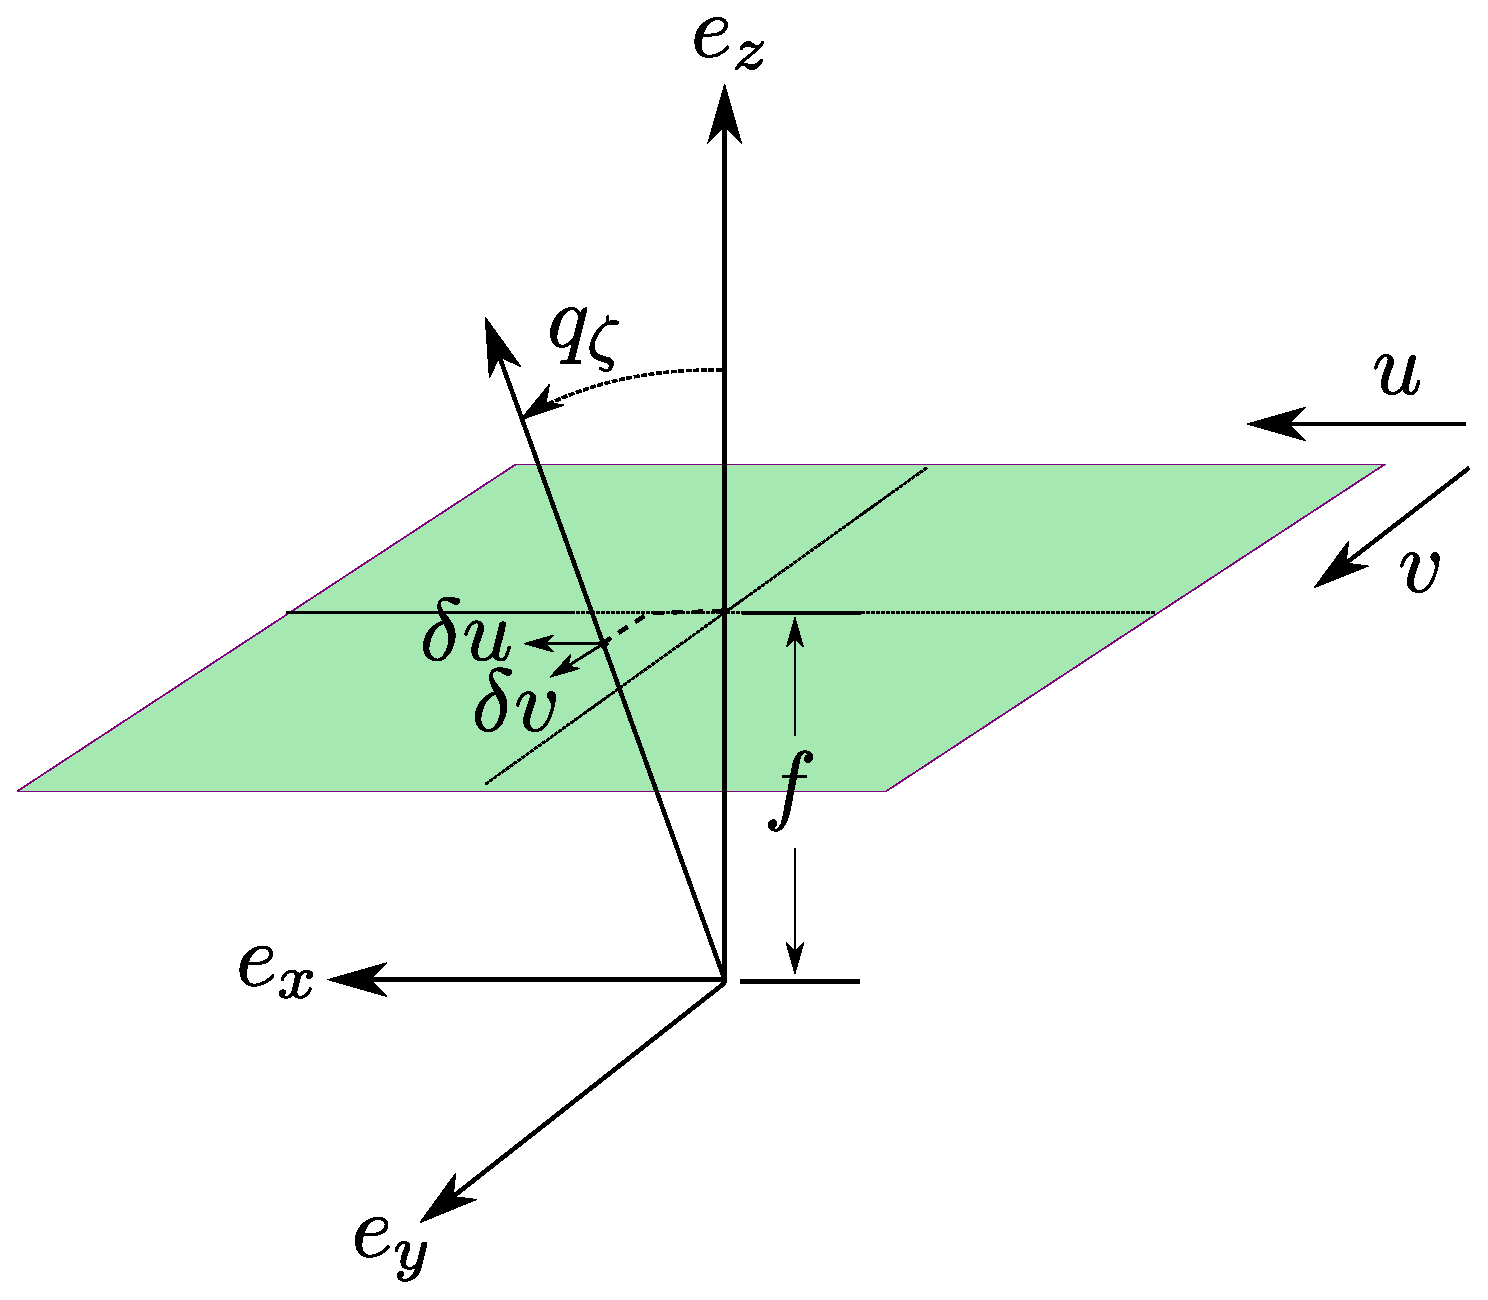
\includegraphics[width=0.8\textwidth]{figures/pixel_vel_diagram}\\
\label{fig:pinhole_camera}
\par\end{centering}

\caption{Pinhole Camera Geometry}
\end{figure}


3D rigid body dynamics require that angular velocity is defined as

\[
\begin{aligned}v & =\omega\times r\end{aligned}
\]


In the case of pixel measurements, the moment arm is the camera z-axis
$e_{z}$ times the focal length $f$ and the velocity vector is given
by $\dot{\lambda}=\tfrac{d\lambda}{dt}$, and the angular velocity
is given by $\omega_{i}=T_{\zeta}\dot{q}_{c}^{\zeta_{i}}$. Therefore
the measurement model is as follows, (using the identity $T_{\zeta}T_{\zeta}^{\top}=I-\zeta\zeta^{\top}$,
and keeping in camera-fixed dynamics to simplify terms):

\begin{equation}
\begin{aligned}h_{\dot{\lambda}}(x,u,\eta_{\dot{\lambda}}) & =-I_{2\times3}\left\lfloor fe_{z}\right\rfloor T_{\zeta}T_{\zeta}^{\top}\left(\rho_{i}\left\lfloor \zeta_{i}^{c}\right\rfloor \left(v_{c/I}^{c}\right)+\omega_{c/I}^{I}\right)\end{aligned}
\label{eq:pixel_velocity_model}
\end{equation}


Differentiating Eq.\ref{eq:pixel_velocity_model} with respect to
the state yields the following Jacobian

\[
H_{\lambda}=\left[\begin{array}{ccccccccc}
0 & \dfrac{\partial h_{\lambda}}{\partial v_{b/i}^{b}} & 0 & 0 & \dfrac{\partial h_{\lambda}}{\partial\beta_{\omega}} & 0 & \cdots & \dfrac{\partial h_{\lambda}}{\partial q_{c}^{\zeta_{i}}} & \dfrac{\partial h_{\lambda}}{\partial\rho_{i}}\end{array}\right]
\]


\[
\begin{aligned}\frac{\partial h_{\dot{\lambda}}}{\partial v_{b/I}^{b}} & =-I_{2\times3}\left\lfloor fe_{z}\right\rfloor \rho_{i}\left\lfloor \zeta_{i}^{c}\right\rfloor \end{aligned}
\]


\[
\begin{aligned}\frac{\partial h_{\dot{\lambda}}}{\partial q_{c}^{\zeta}} & =I_{2\times3}\left\lfloor fe_{z}\right\rfloor \rho_{i}\left\lfloor v_{c/I}^{c}\right\rfloor \left\lfloor \zeta_{i}^{c}\right\rfloor T_{\zeta}\end{aligned}
\]


\[
\begin{aligned}\frac{\partial h_{\dot{\lambda}}}{\partial\rho} & =-I_{2\times3}\left\lfloor fe_{z}\right\rfloor \left\lfloor \zeta_{i}^{c}\right\rfloor \left(v_{c/I}^{c}\right)\end{aligned}
\]


\[
\begin{aligned}\frac{\partial h_{\dot{\lambda}}}{\partial\beta_{\omega}} & =I_{2\times3}\left\lfloor fe_{z}\right\rfloor \left(I-\zeta\zeta^{\top}\right)\left(R\left(q_{b}^{c}\right)-\rho_{i}\left\lfloor \zeta_{i}^{c}\right\rfloor R\left(q_{b}^{c}\right)\left\lfloor p_{cb}^{b}\right\rfloor \right)\end{aligned}
\]



\subsection{Depth Measurement}

Assuming that we had a measurement of depth to a feature, we could
employ the following model:

\[
h_{\rho}(x,u,\eta_{\rho})=\frac{1}{\rho_{i}}
\]


Remembering that $\rho_{i}$ is the inverse depth to feature $i$.
The Jacobian is then as follows:

\[
\frac{\partial h_{\rho}}{\partial\rho_{i}}=-\frac{1}{\rho_{i}^{2}}
\]



\subsection{Inverse Depth Measurement}

Assuming that we had a measurement of inverse depth to a feature,
we could employ the following model:

\[
h_{\rho}(x,u,\eta_{\rho})=\rho_{i}
\]


\[
\frac{\partial h_{\rho}}{\partial\rho_{i}}=1
\]



\subsection{Velocity Measurement}

If we employ an some measurement of body-fixed velocity, 

\[
h_{v}\left(x,u,\eta_{v}\right)=v_{b/I}^{b}+\eta_{v}
\]


\[
\frac{\partial h_{v}}{\partial v_{b/i}^{b}}=I\in\mathbb{R}^{3\times3}
\]



\subsection{Attitude Measurement}

If we employ an some measurement of attitude,

\[
h_{q}\left(x,u,\eta_{v}\right)=q_{I}^{b}+\eta_{q}
\]


\[
\frac{\partial h_{q}}{\partial q_{I}^{b}}=I\in\mathbb{R}^{3\times3}
\]



\subsection{Position Measurement}

If we have some sort of global position measurement, we could employ
the following measurement model:

\[
h_{p}\left(x,u,\eta_{v}\right)=p_{bI}^{I}+\eta_{v}
\]


\[
\frac{\partial h_{p}}{\partial p_{bI}^{I}}=I\in\mathbb{R}^{3\times3}
\]



\section*{Results}

This filter was demonstrated on a quadcopter robot (shown in Figure
\ref{fig:leo}) carrying a monocular Ocam 1CGN-U1MP global shutter
camera and an i7-4500U processor with 8GB of RAM. The onboard IMU
was a statically calibrated MPU6050 recorded at 500Hz. Flight control
was performed using the ROSflight autopilot architecture. Truth was
supplied with a OptiTrack motion-capture system at Brigham Young University.
Camera images and IMU measurements were not directly coupled, so relative
timestamps between the two sensers were estimated to be accurate to
within 1ms, but had small amounts of noise. This is typical of a low-cost
visual-inertial setup.

\begin{figure}[h]
\begin{centering}
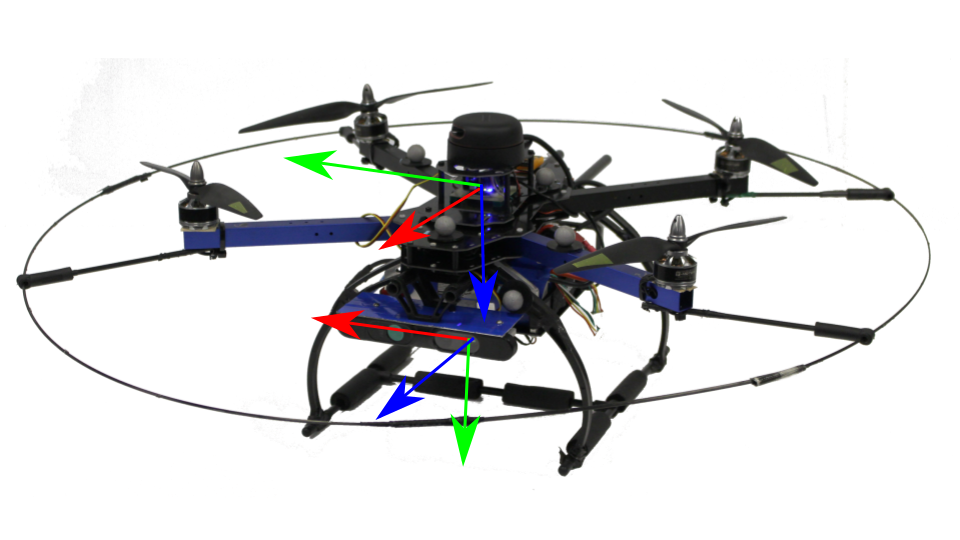
\includegraphics[width=0.8\textwidth]{figures/Leo}\\
\label{fig:leo}
\par\end{centering}

\caption{Multirotor Robot used in hardware demonstration with coordinate frames
for camera and IMU shown. State estimation is performed in the IMU
frame.}
\end{figure}
The Figures \ref{fig:position_results}, \ref{fig:velocity_results}
and \ref{fig:attitude_results} show the performance of our estimator
during this hardware demonstration, while tracking 9 features.

\begin{figure}[h]
\begin{centering}
\includegraphics[width=1\textwidth]{figures/plots/x_euler}
\par\end{centering}

\begin{centering}
\label{fig:attitude_results}
\par\end{centering}

\caption{Attitude estimation results of hardware demonstration in euler angles}
\end{figure}
\begin{figure}[h]
\begin{centering}
\includegraphics[width=1\textwidth]{figures/plots/x_vel}
\par\end{centering}

\begin{centering}
\label{fig:velocity_results}
\par\end{centering}

\caption{Velocity estimation results of hardware demonstration, expressed in
the body frame}
\end{figure}
\begin{figure}[h]
\begin{centering}
\includegraphics[width=1\textwidth]{figures/plots/x_pos}
\par\end{centering}

\begin{centering}
\label{fig:position_results}
\par\end{centering}

\caption{Position estimation results of hardware demonstration, expressed in
inertial coordinates}
\end{figure}



\section*{Conclusion}

In this report we have derived and demonstrated an Extended Kalman
Filter which uses direct updates on the manifold for proper representation
of attitude and feature bearing for a multirotor robot agent. We have
given the closed-form expression for all relevant Jacobians used in
this filter, and the expression for a number of measurement models,
including pixel velocity measurements. We have also merged the use
of the drag model proposed by \citet{Leishman2014b} to improve velocity
estimation within the filter.

\bibliographystyle{upmplainnat}
\bibliography{\string"/home/superjax/Code/bibtex/Visual Odometry\string"}

\end{document}
